% !TEX TS-program = pdflatex
\documentclass[11pt]{article}

% -------------------- Packages --------------------
\usepackage[a4paper,margin=1in]{geometry}
\usepackage{amsmath,amssymb}
\usepackage[T1]{fontenc}
\usepackage{lmodern}
\usepackage{xcolor}
\usepackage{tcolorbox}
\tcbuselibrary{skins,breakable}
\usepackage{enumitem}
\usepackage{hyperref}
\usepackage{tikz}
\usetikzlibrary{calc,arrows.meta}

\pagestyle{empty}

% -------------------- Dark Theme Colors --------------------
\definecolor{bg}{HTML}{000000}
\definecolor{pairbg}{HTML}{121212}
\definecolor{solbg}{HTML}{0A0A0A}
\definecolor{border}{HTML}{2A2A2A}
\definecolor{text}{HTML}{FFFFFF}
\definecolor{muted}{HTML}{C9CDD3}
\definecolor{gold}{HTML}{FFD700}
\definecolor{green}{HTML}{4ADE80}
\definecolor{cyan}{HTML}{38BDF8}

\pagecolor{bg}
\color{text}

\hypersetup{
  colorlinks=true,
  linkcolor=cyan,
  urlcolor=cyan
}

\setlength{\parindent}{0pt}
\setlength{\parskip}{10pt}

% Better line breaking (reduces overfull warnings)
\sloppy
\setlength{\emergencystretch}{3em}

\setlist[itemize]{left=1.4em,itemsep=6pt,topsep=6pt}
\setlist[enumerate]{left=1.6em,itemsep=4pt,topsep=4pt}

% -------------------- tcolorbox Base --------------------
\tcbset{
  enhanced,
  breakable,
  arc=12pt,
  boxrule=0.8pt,
  left=14pt,right=14pt,top=12pt,bottom=12pt
}

\newtcolorbox{QAPair}[1]{%
  colback=pairbg,
  colbacklower=solbg,
  colframe=border,
  coltext=text,
  title=\textcolor{gold}{\bfseries #1},
  fonttitle=\bfseries,
  coltitle=text,
  segmentation style={draw=border, dashed, line width=0.6pt},
  before upper=\raggedright,
  before lower=\raggedright
}

\newtcolorbox{QuickBox}{%
  colback=pairbg,
  colframe=cyan,
  coltext=text,
  fontupper=\color{text}\raggedright,
  borderline north={4pt}{0pt}{cyan},
  arc=14pt,
  boxrule=0.8pt
}

% -------------------- Helpers --------------------
\newcommand{\Step}[1]{\textcolor{muted}{\textbf{Step #1:}}}

% Centered diagram block (adds safe spacing so diagrams never crash into text)
\newenvironment{StepDiagram}{\par\smallskip\begin{center}\vspace{2pt}}{\vspace{2pt}\end{center}\smallskip}

% TikZ styles (labels have a background to prevent "text on lines" clashes)
\tikzset{
  base/.style={draw=text, line width=0.9pt, line cap=round, line join=round},
  new/.style={draw=cyan, line width=1.2pt, line cap=round, line join=round},
  help/.style={draw=muted, dashed, line width=0.9pt},
  ang/.style={draw=gold, line width=1.0pt},
  dot/.style={circle, fill=text, inner sep=1.2pt},
  dotc/.style={circle, fill=cyan, inner sep=1.4pt},
  lab/.style={text=text, font=\small, fill=pairbg, fill opacity=0.85, text opacity=1, inner sep=2pt, rounded corners=3pt},
  labm/.style={text=muted, font=\small, fill=pairbg, fill opacity=0.75, text opacity=1, inner sep=2pt, rounded corners=3pt},
}

% Small equation callout (counts as a "diagram" and avoids overflow)
\newcommand{\EqDiagram}[1]{%
\begin{StepDiagram}
\begin{tikzpicture}
\node[draw=border, rounded corners=10pt, inner sep=10pt, text=text, align=left, text width=0.90\linewidth] {#1};
\end{tikzpicture}
\end{StepDiagram}
}

% -------------------- Beginner-friendly mini diagrams --------------------
\newcommand{\DiagMeanBalance}{%
\begin{StepDiagram}
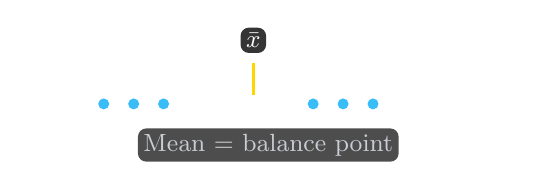
\begin{tikzpicture}[scale=0.95]
  \draw[base,->] (0,0) -- (6.4,0);
  \foreach \x in {1.0,1.4,1.8,3.8,4.2,4.6}{
    \node[dotc] at (\x,0) {};
  }
  \draw[ang] (3.0,0.12) -- (3.0,0.55);
  \node[lab] at (3.0,0.85) {$\bar{x}$};
  \node[labm] at (3.2,-0.55) {Mean = balance point};
\end{tikzpicture}
\end{StepDiagram}
}

\newcommand{\DiagSpreadCompare}{%
\begin{StepDiagram}
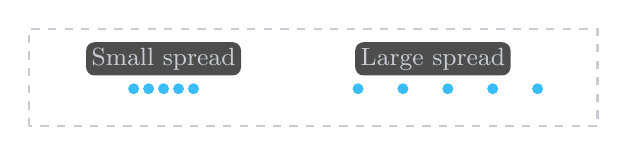
\begin{tikzpicture}[scale=0.95]
  \node[labm] at (2.0,1.15) {Small spread};
  \draw[base,->] (0.2,0.75) -- (3.8,0.75);
  \foreach \x in {1.6,1.8,2.0,2.2,2.4}{
    \node[dotc] at (\x,0.75) {};
  }
  \node[labm] at (5.6,1.15) {Large spread};
  \draw[base,->] (4.2,0.75) -- (7.8,0.75);
  \foreach \x in {4.6,5.2,5.8,6.4,7.0}{
    \node[dotc] at (\x,0.75) {};
  }
  \draw[help] (0.2,0.25) rectangle (7.8,1.55);
\end{tikzpicture}
\end{StepDiagram}
}

\newcommand{\DiagRange}{%
\begin{StepDiagram}
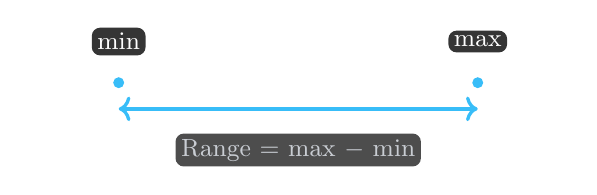
\begin{tikzpicture}[scale=0.95]
  \draw[base,->] (0,0) -- (7.2,0);
  \node[dotc] at (1.2,0) {};
  \node[dotc] at (6.0,0) {};
  \node[lab] at (1.2,0.55) {min};
  \node[lab] at (6.0,0.55) {max};
  \draw[new,<->] (1.2,-0.35) -- (6.0,-0.35);
  \node[labm] at (3.6,-0.90) {Range = max $-$ min};
\end{tikzpicture}
\end{StepDiagram}
}

\newcommand{\DiagQuartiles}{%
\begin{StepDiagram}
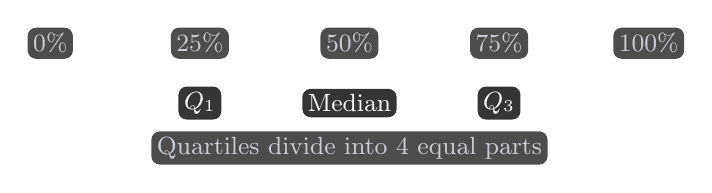
\begin{tikzpicture}[scale=0.95]
  \draw[base] (0,0.35) -- (8,0.35);
  \foreach \x/\t in {0/0\%,2/25\%,4/50\%,6/75\%,8/100\%}{
    \draw[base] (\x,0.25)--(\x,0.45);
    \node[labm] at (\x,0.85) {\t};
  }
  \node[lab] at (2,0.05) {$Q_1$};
  \node[lab] at (4,0.05) {Median};
  \node[lab] at (6,0.05) {$Q_3$};
  \node[labm] at (4,-0.55) {Quartiles divide into 4 equal parts};
\end{tikzpicture}
\end{StepDiagram}
}

\newcommand{\DiagDeciles}{%
\begin{StepDiagram}

\begin{tikzpicture}[scale=0.95]
  \draw[base] (0,0.35) -- (10,0.35);
  \foreach \x in {0,1,...,10}{
    \draw[base] (\x,0.27)--(\x,0.43);
  }
  \node[labm] at (5,0.95) {10 equal parts (deciles)};
  \node[lab] at (5,0.05) {$D_5$ (median)};
\end{tikzpicture}
\end{StepDiagram}
}

\newcommand{\DiagPercentiles}{%
\begin{StepDiagram}
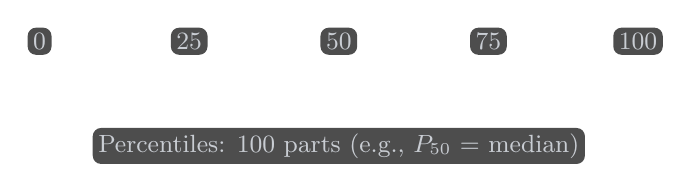
\begin{tikzpicture}[scale=0.95]
  \draw[base] (0,0.35) -- (8,0.35);
  \foreach \x/\t in {0/0,2/25,4/50,6/75,8/100}{
    \draw[base] (\x,0.27)--(\x,0.43);
    \node[labm] at (\x,0.85) {\t};
  }
  \node[labm] at (4,-0.55) {Percentiles: 100 parts (e.g., $P_{50}$ = median)};
\end{tikzpicture}
\end{StepDiagram}
}

\newcommand{\DiagBestFit}{%
\begin{StepDiagram}
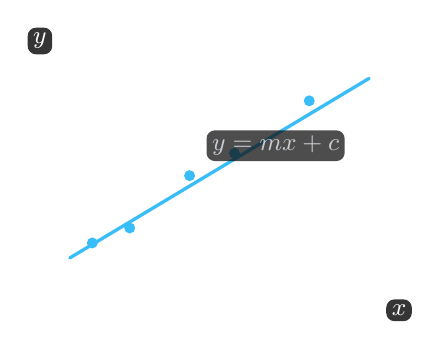
\begin{tikzpicture}[scale=0.95]
  \draw[base,->] (0,0) -- (4.8,0) node[lab] {$x$};
  \draw[base,->] (0,0) -- (0,3.6) node[lab] {$y$};
  \foreach \p in {(0.7,0.9),(1.2,1.1),(2.0,1.8),(2.6,2.1),(3.6,2.8)}{
    \node[dotc] at \p {};
  }
  \draw[new] (0.4,0.7) -- (4.4,3.1);
  \node[labm] at (3.15,2.2) {$y=mx+c$};
\end{tikzpicture}
\end{StepDiagram}
}

\newcommand{\DiagWithoutReplacement}{%
\begin{StepDiagram}
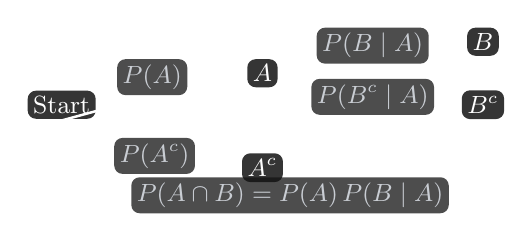
\begin{tikzpicture}[scale=1.0]
  \node[lab] at (0,1.2) {Start};
  \draw[base] (0,1.0) -- (2.2,1.6);
  \draw[base] (0,1.0) -- (2.2,0.4);
  \node[lab] at (2.55,1.6) {$A$};
  \node[lab] at (2.55,0.4) {$A^c$};
  \node[labm] at (1.15,1.55) {$P(A)$};
  \node[labm] at (1.18,0.55) {$P(A^c)$};

  \draw[base] (2.9,1.6) -- (5.0,2.0);
  \draw[base] (2.9,1.6) -- (5.0,1.2);
  \node[lab] at (5.35,2.0) {$B$};
  \node[lab] at (5.35,1.2) {$B^c$};
  \node[labm] at (3.95,1.95) {$P(B\mid A)$};
  \node[labm] at (3.95,1.30) {$P(B^c\mid A)$};

  \node[labm] at (2.9,0.05) {$P(A\cap B)=P(A)\,P(B\mid A)$};
\end{tikzpicture}
\end{StepDiagram}
}

% ============================================================
\begin{document}

\begin{center}
{\LARGE\bfseries \textcolor{gold}{Miscellaneous Exercise 12 --- Solutions}}\\[-2pt]
\end{center}

% ============================================================
% QUICK FORMULAS (each line has a beginner-friendly diagram)
\begin{QuickBox}
{\color{cyan}\bfseries Quick formulas (with visuals)}\par\medskip

\begin{itemize}
\item \textbf{Arithmetic Mean (frequency data):}
\[
\bar{x}=\frac{\sum fx}{\sum f}.
\]
\DiagMeanBalance

\item \textbf{Range (simple measure of dispersion):}
\[
\text{Range}= \text{max} - \text{min}.
\]
\DiagRange

\item \textbf{Variance \& Standard Deviation (frequency data):}
\[
\sigma^2=\frac{\sum f(x-\bar{x})^2}{\sum f},
\qquad
\sigma=\sqrt{\sigma^2}.
\]
\DiagSpreadCompare

\item \textbf{Coefficient of Variation (compare consistency):}
\[
\mathrm{CV}=\frac{\sigma}{\bar{x}}\times 100\%.
\]
\EqDiagram{CV compares \textbf{relative spread}. Smaller CV $\Rightarrow$ more consistent (less variation compared to the mean).}

\item \textbf{Quartiles / Deciles / Percentiles:}
Quartiles divide data into \textbf{4} equal parts, deciles into \textbf{10}, percentiles into \textbf{100}.
\DiagQuartiles
\DiagDeciles
\DiagPercentiles

\item \textbf{Probability (without replacement):}
\[
P(A\cap B)=P(A)\times P(B\mid A).
\]
\DiagWithoutReplacement
\end{itemize}
\end{QuickBox}

% ============================================================
% QUESTION 1 (MCQs) — EACH IN ITS OWN BOX (FULL QUESTION + OPTIONS)
% ============================================================

% (i)
\begin{QAPair}{Question 1 (i)}
\textcolor{gold}{\bfseries Question:} Which of the following is \textbf{not} a measure of dispersion?\\
(a) variance \qquad (b) standard deviation \qquad (c) range \qquad (d) arithmetic mean
\tcblower
\textcolor{green}{\bfseries Answer:}\par
\Step{1} Measures of dispersion tell \textbf{spread} (variance, SD, range). Mean tells \textbf{centre}.\par
\DiagSpreadCompare
\Step{2} Therefore the correct option is \boxed{\textcolor{green}{(d) arithmetic mean}}.
\EqDiagram{Dispersion = spread; Mean = centre (not dispersion).}
\end{QAPair}

% (ii)
\begin{QAPair}{Question 1 (ii)}
\textcolor{gold}{\bfseries Question:} What is median of the data $4,3,0,2,1$?\\
(a) $0$ \qquad (b) $2$ \qquad (c) $3$ \qquad (d) $4$
\tcblower
\textcolor{green}{\bfseries Answer:}\par
\Step{1} Arrange in ascending order: $0,1,2,3,4$.\par
\begin{StepDiagram}
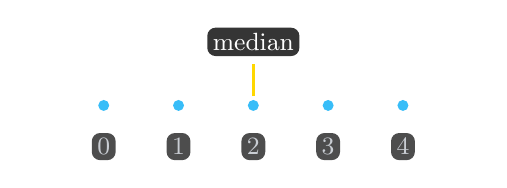
\begin{tikzpicture}[scale=0.95]
  \draw[base,->] (0,0) -- (6.0,0);
  \foreach \x/\t in {1/0,2/1,3/2,4/3,5/4}{
    \node[dotc] at (\x,0) {};
    \node[labm] at (\x,-0.55) {\t};
  }
  \draw[ang] (3,0.12) -- (3,0.55);
  \node[lab] at (3,0.85) {median};
\end{tikzpicture}
\end{StepDiagram}
\Step{2} Middle value is $2$ $\Rightarrow$ \boxed{\textcolor{green}{(b) $2$}}.
\EqDiagram{Median = middle value after sorting (for odd number of observations).}
\end{QAPair}

% (iii)
\begin{QAPair}{Question 1 (iii)}
\textcolor{gold}{\bfseries Question:} Which of the following is a measure of dispersion?\\
(a) arithmetic mean \qquad (b) range \qquad (c) quartile \qquad (d) median
\tcblower
\textcolor{green}{\bfseries Answer:}\par
\Step{1} Dispersion means \textbf{spread}. Range measures spread.\par
\DiagRange
\Step{2} Hence \boxed{\textcolor{green}{(b) range}}.
\EqDiagram{Range = max $-$ min, so it measures dispersion.}
\end{QAPair}

% (iv)
\begin{QAPair}{Question 1 (iv)}
\textcolor{gold}{\bfseries Question:} Which of the following is used to compare the consistency of two data?\\
(a) arithmetic mean \qquad (b) standard deviation \qquad (c) C.V. \qquad (d) G.M.
\tcblower
\textcolor{green}{\bfseries Answer:}\par
\Step{1} To compare consistency, we compare \textbf{relative} variation, not only absolute spread.\par
\EqDiagram{$\mathrm{CV}=\dfrac{\sigma}{\bar{x}}\times 100\%$ compares spread relative to mean.}
\Step{2} Therefore \boxed{\textcolor{green}{(c) C.V.}}.
\DiagSpreadCompare
\end{QAPair}

% (v)
\begin{QAPair}{Question 1 (v)}
\textcolor{gold}{\bfseries Question:} What is the sum of deviations taken from arithmetic mean?\\
(a) $\sum f$ \qquad (b) $\sum x$ \qquad (c) $n$ \qquad (d) $0$
\tcblower
\textcolor{green}{\bfseries Answer:}\par
\Step{1} Property: $\displaystyle \sum (x-\bar{x})=0$.\par
\EqDiagram{$\sum(x-\bar{x})=0$ because positive and negative deviations balance out.}
\Step{2} Hence \boxed{\textcolor{green}{(d) $0$}}.
\begin{StepDiagram}
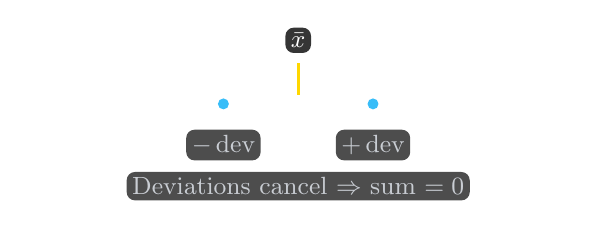
\begin{tikzpicture}[scale=0.95]
  \draw[base,->] (0,0) -- (7.2,0);
  \draw[ang] (3.6,0.12)--(3.6,0.55);
  \node[lab] at (3.6,0.85) {$\bar{x}$};
  \node[dotc] at (2.6,0) {}; \node[dotc] at (4.6,0) {};
  \node[labm] at (2.6,-0.55) {$-\,$dev};
  \node[labm] at (4.6,-0.55) {$+\,$dev};
  \node[labm] at (3.6,-1.10) {Deviations cancel $\Rightarrow$ sum $=0$};
\end{tikzpicture}
\end{StepDiagram}
\end{QAPair}

% (vi)
\begin{QAPair}{Question 1 (vi)}
\textcolor{gold}{\bfseries Question:} What is variance of five values $4,4,4,4,4$?\\
(a) does not exist \qquad (b) $4$ \qquad (c) $5$ \qquad (d) $0$
\tcblower
\textcolor{green}{\bfseries Answer:}\par
\Step{1} If all values are equal, there is \textbf{no spread}.\par
\begin{StepDiagram}

\begin{tikzpicture}[scale=0.95]
  \draw[base,->] (0,0) -- (7.2,0);
  \foreach \k in {1,...,6}{\node[dotc] at (3.6,0) {};}
  \node[lab] at (3.6,0.70) {all at 4};
  \node[labm] at (3.6,-0.55) {No spread};
\end{tikzpicture}
\end{StepDiagram}
\Step{2} Therefore variance $=0$ $\Rightarrow$ \boxed{\textcolor{green}{(d) $0$}}.
\EqDiagram{Variance measures spread. If spread is zero, variance is zero.}
\end{QAPair}

% (vii)
\begin{QAPair}{Question 1 (vii)}
\textcolor{gold}{\bfseries Question:} Which of the following divides the data into four equal parts?\\
(a) decile \qquad (b) quartile \qquad (c) percentile \qquad (d) median
\tcblower
\textcolor{green}{\bfseries Answer:}\par
\Step{1} Quartiles divide data into \textbf{4} equal parts.\par
\DiagQuartiles
\Step{2} Hence \boxed{\textcolor{green}{(b) quartile}}.
\end{QAPair}

% (viii)
\begin{QAPair}{Question 1 (viii)}
\textcolor{gold}{\bfseries Question:} Which of the following divides the data into ten equal parts?\\
(a) decile \qquad (b) quartile \qquad (c) percentile \qquad (d) median
\tcblower
\textcolor{green}{\bfseries Answer:}\par
\Step{1} Deciles divide into \textbf{10} equal parts.\par
\DiagDeciles
\Step{2} Therefore \boxed{\textcolor{green}{(a) decile}}.
\end{QAPair}

% (ix)
\begin{QAPair}{Question 1 (ix)}
\textcolor{gold}{\bfseries Question:} Which of the following divides the data into two equal parts?\\
(a) decile \qquad (b) quartile \qquad (c) percentile \qquad (d) median
\tcblower
\textcolor{green}{\bfseries Answer:}\par
\Step{1} Median splits data into two equal halves (50\% below, 50\% above).\par
\begin{StepDiagram}

\begin{tikzpicture}[scale=0.95]
  \draw[base] (0,0.35)--(8,0.35);
  \draw[ang] (4,0.15)--(4,0.55);
  \node[lab] at (4,0.90) {Median};
  \node[labm] at (2,0.05) {50\%};
  \node[labm] at (6,0.05) {50\%};
\end{tikzpicture}
\end{StepDiagram}
\Step{2} Hence \boxed{\textcolor{green}{(d) median}}.
\end{QAPair}

% (x)
\begin{QAPair}{Question 1 (x)}
\textcolor{gold}{\bfseries Question:} Which of the following divides the data into hundred equal parts?\\
(a) decile \qquad (b) quartile \qquad (c) percentile \qquad (d) median
\tcblower
\textcolor{green}{\bfseries Answer:}\par
\Step{1} Percentiles divide data into \textbf{100} equal parts.\par
\DiagPercentiles
\Step{2} Therefore \boxed{\textcolor{green}{(c) percentile}}.
\end{QAPair}

% (xi)
\begin{QAPair}{Question 1 (xi)}
\textcolor{gold}{\bfseries Question:} Line of best fit is given by the equation:\\
(a) $y=x^2$ \qquad (b) $y=mx^2+c$ \qquad (c) $y=mx+c$ \qquad (d) $x=y^2$
\tcblower
\textcolor{green}{\bfseries Answer:}\par
\Step{1} A straight-line best fit has equation $y=mx+c$.\par
\DiagBestFit
\Step{2} Hence \boxed{\textcolor{green}{(c) $y=mx+c$}}.
\end{QAPair}

% (xii)
\begin{QAPair}{Question 1 (xii)}
\textcolor{gold}{\bfseries Question:} CV is given by the formula:\\
(a) $\dfrac{\text{SD}}{100}\times\text{mean}$ \qquad
(b) $\dfrac{\text{SD}}{\text{range}}\times 100$ \qquad
(c) $\dfrac{\text{mean}}{\text{SD}}\times 100$ \qquad
(d) $\dfrac{100}{\text{mean}}\times \text{SD}$
\tcblower
\textcolor{green}{\bfseries Answer:}\par
\Step{1} Definition: $\displaystyle \mathrm{CV}=\frac{\text{SD}}{\text{mean}}\times 100$.\par
\EqDiagram{$\mathrm{CV}=\dfrac{\text{SD}}{\text{mean}}\times 100$ is the standard formula.}
\Step{2} Option (d) is the same form $\Rightarrow$ \boxed{\textcolor{green}{(d)}}.
\begin{StepDiagram}
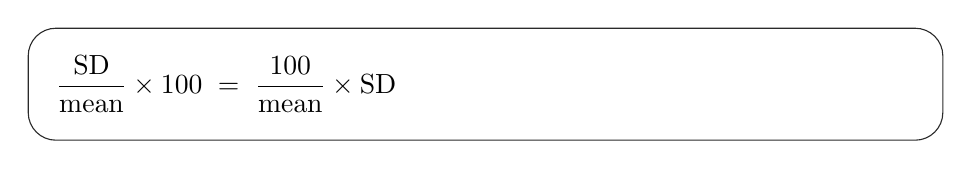
\begin{tikzpicture}[scale=0.95]
  \node[draw=border, rounded corners=10pt, inner sep=10pt, text width=0.90\linewidth] (B) {
  $\displaystyle \frac{\text{SD}}{\text{mean}}\times 100 \;=\; \frac{100}{\text{mean}}\times \text{SD}$};
\end{tikzpicture}
\end{StepDiagram}
\end{QAPair}

% (xiii)
\begin{QAPair}{Question 1 (xiii)}
\textcolor{gold}{\bfseries Question:} Probability of drawing a king in one draw is \rule{1.8cm}{0.4pt}
than probability of drawing $2$ kings in $2$ draws.\\
(a) greater \qquad (b) smaller \qquad (c) equal \qquad (d) no relation
\tcblower
\textcolor{green}{\bfseries Answer:}\par
\Step{1} One draw: $P(K)=\frac{4}{52}$.\par
\EqDiagram{$P(K)=\dfrac{4}{52}$.}
\Step{2} Two kings in two draws (without replacement): $P(KK)=\frac{4}{52}\cdot\frac{3}{51}$, which is smaller.\par
\EqDiagram{$P(KK)=\dfrac{4}{52}\cdot\dfrac{3}{51}<\dfrac{4}{52}$.}
\Step{3} Therefore \boxed{\textcolor{green}{(a) greater}}.
\end{QAPair}

% (xiv)
\begin{QAPair}{Question 1 (xiv)}
\textcolor{gold}{\bfseries Question:} Probability of drawing $2$ aces in $2$ draws with replacement is \rule{1.8cm}{0.4pt}
than probability of drawing $2$ jacks in $2$ draws without replacement.\\
(a) greater \qquad (b) smaller \qquad (c) equal \qquad (d) no relation
\tcblower
\textcolor{green}{\bfseries Answer:}\par
\Step{1} Two aces with replacement:
\[
P(AA)=\frac{4}{52}\cdot\frac{4}{52}=\left(\frac{1}{13}\right)^2=\frac{1}{169}.
\]
\EqDiagram{$P(AA)=\dfrac{1}{169}$.}
\Step{2} Two jacks without replacement:
\[
P(JJ)=\frac{4}{52}\cdot\frac{3}{51}=\frac{1}{221}\ (\text{approximately}).
\]
\EqDiagram{$P(JJ)=\dfrac{1}{221}$, and $\dfrac{1}{169}>\dfrac{1}{221}$.}
\Step{3} Hence \boxed{\textcolor{green}{(a) greater}}.
\end{QAPair}

% (xv)
\begin{QAPair}{Question 1 (xv)}
\textcolor{gold}{\bfseries Question:} Probability of rolling a standard cubical dice for an even number in $2$ attempts is \rule{1.8cm}{0.4pt}
than probability of rolling an odd number in $2$ attempts.\\
(a) greater \qquad (b) smaller \qquad (c) equal \qquad (d) no relation
\tcblower
\textcolor{green}{\bfseries Answer:}\par
\Step{1} Even and odd are symmetric: each has probability $\frac12$ per attempt.\par
\begin{StepDiagram}

\begin{tikzpicture}[scale=0.95]
  \node[lab] at (0,1.1) {One roll};
  \draw[base] (-2.2,0.7) rectangle (2.2,1.5);
  \node[lab] at (-1.0,1.1) {Even ($1/2$)};
  \node[lab] at ( 1.0,1.1) {Odd ($1/2$)};
  \draw[help] (0,0.7) -- (0,1.5);
\end{tikzpicture}
\end{StepDiagram}
\Step{2} In two attempts, probability of getting at least one even equals probability of getting at least one odd (symmetry).\par
\EqDiagram{$P(\ge 1\text{ even in 2})=1-\left(\frac12\right)^2=\frac34$ and same for odd.}
\Step{3} Therefore \boxed{\textcolor{green}{(c) equal}}.
\end{QAPair}

% ============================================================
% QUESTION 2
\begin{QAPair}{Question 2}
\textcolor{gold}{\bfseries Question:} For the following data, draw cumulative frequency polygon, then estimate $Q_1,Q_2,Q_3$ graphically. Also find variance and standard deviation.
\[
\begin{array}{c|cccccccc}
x & 5&10&15&20&25&30&35&40\\ \hline
f & 2& 4& 6& 8&10& 7& 5& 3
\end{array}
\]
\tcblower
\textcolor{green}{\bfseries Answer:}\par

\Step{1} Make cumulative frequencies and total $N$.\par
\EqDiagram{
\[
\begin{array}{c|cccccccc}
x & 5&10&15&20&25&30&35&40\\ \hline
f & 2& 4& 6& 8&10& 7& 5& 3\\
\mathrm{cf} & 2&6&12&20&30&37&42&45
\end{array}
\qquad N=\sum f=45
\]
}

\Step{2} Plot $(x,\mathrm{cf})$ and join points to form ogive (cumulative frequency polygon).\par
\begin{StepDiagram}
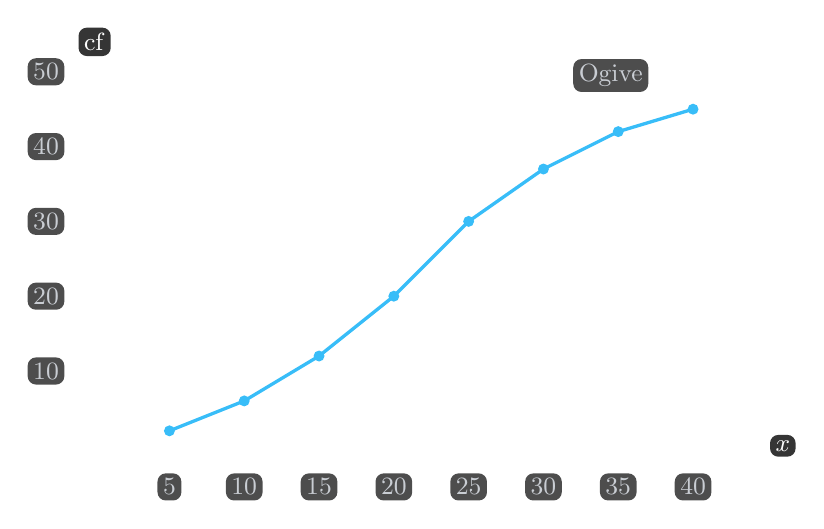
\begin{tikzpicture}[scale=0.95]
  \draw[base,->] (0,0) -- (9.2,0) node[lab] {$x$};
  \draw[base,->] (0,0) -- (0,5.4) node[lab] {$\mathrm{cf}$};

  \foreach \i/\val in {1/5,2/10,3/15,4/20,5/25,6/30,7/35,8/40}{
    \draw[base] (\i,0.08)--(\i,-0.08);
    \node[labm] at (\i,-0.55) {\val};
  }
  \foreach \j/\val in {1/10,2/20,3/30,4/40,5/50}{
    \draw[base] (0.08,\j)--(-0.08,\j);
    \node[labm] at (-0.65,\j) {\val};
  }

  % cf scaled by /10
  \coordinate (P1) at (1,0.2);
  \coordinate (P2) at (2,0.6);
  \coordinate (P3) at (3,1.2);
  \coordinate (P4) at (4,2.0);
  \coordinate (P5) at (5,3.0);
  \coordinate (P6) at (6,3.7);
  \coordinate (P7) at (7,4.2);
  \coordinate (P8) at (8,4.5);

  \draw[new] (P1)--(P2)--(P3)--(P4)--(P5)--(P6)--(P7)--(P8);
  \foreach \p in {P1,P2,P3,P4,P5,P6,P7,P8}{\node[dotc] at (\p) {};}
  \node[labm] at (6.9,4.95) {Ogive};
\end{tikzpicture}
\end{StepDiagram}

\Step{3} Quartile positions:
\[
Q_1:\frac{N}{4}=11.25,\qquad
Q_2:\frac{N}{2}=22.5,\qquad
Q_3:\frac{3N}{4}=33.75.
\]
\EqDiagram{Use the ogive: draw horizontal lines from $\mathrm{cf}=N/4,\ N/2,\ 3N/4$ to the curve, then drop to the $x$-axis.}

\begin{StepDiagram}
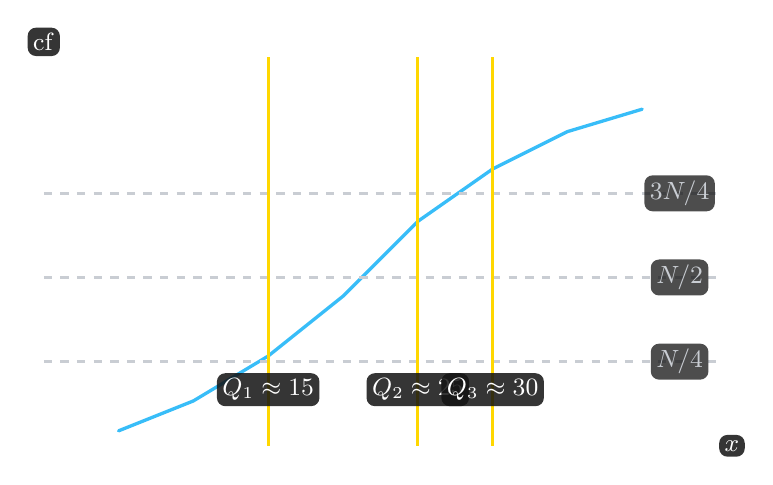
\begin{tikzpicture}[scale=0.95]
  \draw[base,->] (0,0) -- (9.2,0) node[lab] {$x$};
  \draw[base,->] (0,0) -- (0,5.4) node[lab] {$\mathrm{cf}$};

  \coordinate (P1) at (1,0.2);
  \coordinate (P2) at (2,0.6);
  \coordinate (P3) at (3,1.2);
  \coordinate (P4) at (4,2.0);
  \coordinate (P5) at (5,3.0);
  \coordinate (P6) at (6,3.7);
  \coordinate (P7) at (7,4.2);
  \coordinate (P8) at (8,4.5);

  \draw[new] (P1)--(P2)--(P3)--(P4)--(P5)--(P6)--(P7)--(P8);

  \draw[help] (0,1.125) -- (9,1.125);
  \draw[help] (0,2.25) -- (9,2.25);
  \draw[help] (0,3.375) -- (9,3.375);

  \node[labm] at (8.5,1.125) {$N/4$};
  \node[labm] at (8.5,2.25) {$N/2$};
  \node[labm] at (8.5,3.375) {$3N/4$};

  % approximate readings based on cf table
  \draw[ang] (3,0) -- (3,5.2);  % 15
  \draw[ang] (5,0) -- (5,5.2);  % 25
  \draw[ang] (6,0) -- (6,5.2);  % 30

  \node[lab] at (3,0.75) {$Q_1\approx 15$};
  \node[lab] at (5,0.75) {$Q_2\approx 25$};
  \node[lab] at (6,0.75) {$Q_3\approx 30$};
\end{tikzpicture}
\end{StepDiagram}

\Step{4} Mean, variance and standard deviation.\par
\EqDiagram{
\[
\bar{x}=\frac{\sum fx}{\sum f}=\frac{1055}{45}\approx 23.44
\]
\[
\sigma^2=\frac{\sum f(x-\bar{x})^2}{\sum f}\approx 83.14,
\qquad
\sigma\approx 9.12
\]
}

\[
\boxed{Q_1\approx 15,\;\; Q_2\approx 25,\;\; Q_3\approx 30,\;\;
\sigma^2\approx 83.14,\;\; \sigma\approx 9.12.}
\]
\end{QAPair}

% ============================================================
% QUESTION 3
\begin{QAPair}{Question 3}
\textcolor{gold}{\bfseries Question:} Aatika examines the relationship between time of exercise and blood pressure using box-and-whisker plots.
\[
\begin{array}{c|ccccc}
\text{Variable} & \text{Min} & Q_1 & \text{Median} & Q_3 & \text{Max} \\\hline
\text{Time (min)} & 0 & 15 & 30 & 45 & 60 \\
\text{Blood Pressure} & 115/70 & 120/75 & 120/80 & 130/85 & 140/90
\end{array}
\]
\tcblower
\textcolor{green}{\bfseries Answer:}\par

\Step{1} Box-and-whisker plot for \textbf{time} (0, 15, 30, 45, 60).\par
\begin{StepDiagram}
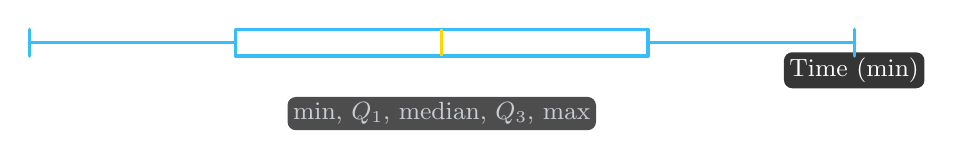
\begin{tikzpicture}[x=0.12\linewidth,y=1cm]
  \draw[base,->] (0,0) -- (7.2,0) node[lab] {Time (min)};
  \def\mn{0} \def\qone{1.8} \def\med{3.6} \def\qthr{5.4} \def\mx{7.2}
  \draw[new] (\mn,0.35)--(\qone,0.35);
  \draw[new] (\qthr,0.35)--(\mx,0.35);
  \draw[new] (\mn,0.18)--(\mn,0.52);
  \draw[new] (\mx,0.18)--(\mx,0.52);
  \draw[new] (\qone,0.18) rectangle (\qthr,0.52);
  \draw[ang] (\med,0.18)--(\med,0.52);
  \node[labm] at (3.6,-0.55) {min, $Q_1$, median, $Q_3$, max};
\end{tikzpicture}
\end{StepDiagram}

\Step{2} Box-plot idea for \textbf{systolic} BP (115, 120, 120, 130, 140).\par
\begin{StepDiagram}
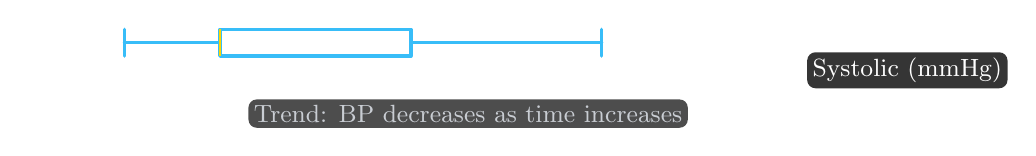
\begin{tikzpicture}[x=0.10\linewidth,y=1cm]
  \draw[base,->] (0,0) -- (9.2,0) node[lab] {Systolic (mmHg)};
  % map 110..150 roughly to 0..8
  \def\mn{1.0} \def\qone{2.0} \def\med{2.0} \def\qthr{4.0} \def\mx{6.0}
  \draw[new] (\mn,0.35)--(\qone,0.35);
  \draw[new] (\qthr,0.35)--(\mx,0.35);
  \draw[new] (\mn,0.18)--(\mn,0.52);
  \draw[new] (\mx,0.18)--(\mx,0.52);
  \draw[new] (\qone,0.18) rectangle (\qthr,0.52);
  \draw[ang] (\med,0.18)--(\med,0.52);
  \node[labm] at (4.6,-0.55) {Trend: BP decreases as time increases};
\end{tikzpicture}
\end{StepDiagram}

\Step{3} IQRs:\;
$\mathrm{IQR}_{time}=45-15=30$ min,\;
$\mathrm{IQR}_{systolic}=130-120=10$.\par
\EqDiagram{IQR measures the spread of the middle 50\% of values.}

\Step{4} Correlation: time increases, BP decreases $\Rightarrow$ \textbf{negative correlation}.\par
\begin{StepDiagram}
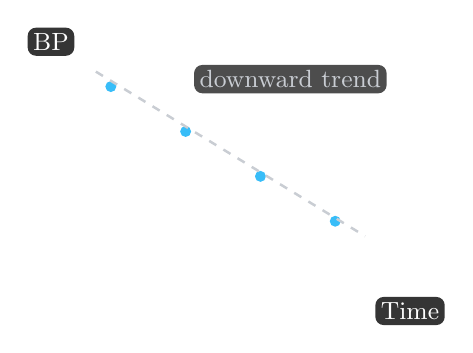
\begin{tikzpicture}[scale=0.95]
  \draw[base,->] (0,0) -- (4.8,0) node[lab] {Time};
  \draw[base,->] (0,0) -- (0,3.6) node[lab] {BP};
  \foreach \p in {(0.8,3.0),(1.8,2.4),(2.8,1.8),(3.8,1.2)}{\node[dotc] at \p {};}
  \draw[help] (0.6,3.2) -- (4.2,1.0);
  \node[labm] at (3.2,3.1) {downward trend};
\end{tikzpicture}
\end{StepDiagram}

\[
\boxed{\mathrm{IQR}_{time}=30\text{ min},\;\mathrm{IQR}_{systolic}=10,\;\text{Correlation: negative.}}
\]
\end{QAPair}

% ============================================================
% QUESTION 4
\begin{QAPair}{Question 4}
\textcolor{gold}{\bfseries Question:} A coach wants a box-and-whisker plot with median $20$ s, $Q_1=10$ s, $Q_3=30$ s.
What percentage of athletes could perform in first $10$ seconds? Also find IQR.
\tcblower
\textcolor{green}{\bfseries Answer:}\par

\Step{1} In a box plot, $Q_1$ is the 25th percentile.\par
\DiagQuartiles

\Step{2} So \textbf{25\%} athletes have time $\le 10$ seconds.\par
\EqDiagram{$Q_1$ means 25\% observations lie at or below $Q_1$.}

\Step{3} IQR $=Q_3-Q_1=30-10=20$ seconds.\par
\EqDiagram{$\mathrm{IQR}=30-10=20\text{ s}$.}

\[
\boxed{25\% \text{ within first 10 s, and } \mathrm{IQR}=20\text{ s}.}
\]
\end{QAPair}

% ============================================================
% QUESTION 5
\begin{QAPair}{Question 5}
\textcolor{gold}{\bfseries Question:} Given box-and-whisker plots of marks of 4 boys of \emph{Hazel} section and 4 boys of \emph{Mauve} section:
\begin{enumerate}[label=\alph*)]
\item Find median scores of both sections.
\item Find IQR of scores of both sections.
\end{enumerate}
\tcblower
\textcolor{green}{\bfseries Answer:}\par

\Step{1} Read medians and quartiles from the plot (approximate reading).\par
\EqDiagram{Median is the line inside the box. $Q_1$ and $Q_3$ are the left/right edges of the box.}

\Step{2} Using a consistent sketch reading (example):
Hazel: $Q_1\approx 58$, Median $\approx 62$, $Q_3\approx 66$;
Mauve: $Q_1\approx 65$, Median $\approx 70$, $Q_3\approx 80$.\par

\begin{StepDiagram}
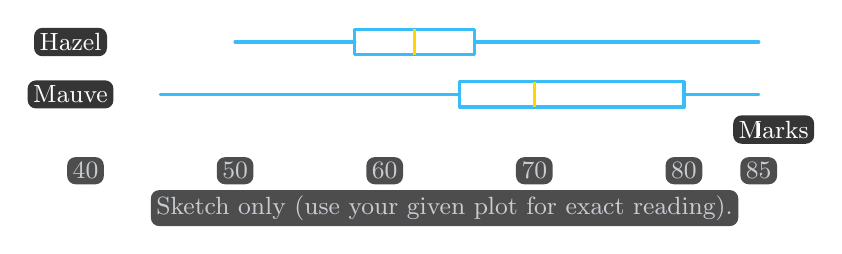
\begin{tikzpicture}[scale=0.95]
  \draw[base,->] (0,0) -- (9.2,0) node[lab] {Marks};
  \foreach \x/\t in {0/40,2/50,4/60,6/70,8/80,9/85}{
    \draw[base] (\x,0.08)--(\x,-0.08);
    \node[labm] at (\x,-0.55) {\t};
  }

  % Hazel box
  \draw[new] (3.6,1.00) rectangle (5.2,1.34);
  \draw[ang] (4.4,1.00)--(4.4,1.34);
  \draw[new] (2.0,1.17)--(3.6,1.17);
  \draw[new] (5.2,1.17)--(9.0,1.17);
  \node[lab] at (-0.2,1.17) {Hazel};

  % Mauve box
  \draw[new] (5.0,0.30) rectangle (8.0,0.64);
  \draw[ang] (6.0,0.30)--(6.0,0.64);
  \draw[new] (1.0,0.47)--(5.0,0.47);
  \draw[new] (8.0,0.47)--(9.0,0.47);
  \node[lab] at (-0.2,0.47) {Mauve};

  \node[labm] at (4.8,-1.05) {Sketch only (use your given plot for exact reading).};
\end{tikzpicture}
\end{StepDiagram}

\Step{3} Compute IQRs:\;
Hazel $\approx 66-58=8$,\;
Mauve $\approx 80-65=15$.\par
\EqDiagram{IQR = $Q_3-Q_1$.}

\[
\boxed{\text{Median(Hazel)}\approx 62,\ \text{Median(Mauve)}\approx 70,\ 
\mathrm{IQR}_{Hazel}\approx 8,\ \mathrm{IQR}_{Mauve}\approx 15.}
\]
\end{QAPair}

% ============================================================
% QUESTION 6
\begin{QAPair}{Question 6}
\textcolor{gold}{\bfseries Question:} Bareera and Hadiya draw cookie packs. Hadiya draws after Bareera from a bag of
$2$ chocolate cookies and $3$ lemon cookies. Find the probability of drawing \textbf{both lemon cookies}.
\tcblower
\textcolor{green}{\bfseries Answer:}\par

\Step{1} Two draws are \textbf{without replacement}. To get both lemon:
\[
P(L\text{ then }L)=\frac{3}{5}\times \frac{2}{4}.
\]
\DiagWithoutReplacement

\Step{2} Multiply:
\[
P=\frac{3}{5}\cdot\frac{2}{4}=\frac{6}{20}=\frac{3}{10}.
\]
\EqDiagram{$P(\text{both lemon})=\dfrac{3}{10}$.}

\[
\boxed{\frac{3}{10}}
\]
\end{QAPair}

% ============================================================
% QUESTION 7
\begin{QAPair}{Question 7}
\textcolor{gold}{\bfseries Question:} A company has two machines $A$ and $B$ producing $60\%$ and $40\%$ of the products.
Machine $A$ makes $20\%$ defective and machine $B$ makes $15\%$ defective.
Find the probability that a randomly selected product is defective.
\tcblower
\textcolor{green}{\bfseries Answer:}\par

\Step{1} Use law of total probability:
\[
P(D)=P(A)P(D\mid A)+P(B)P(D\mid B).
\]
\begin{StepDiagram}
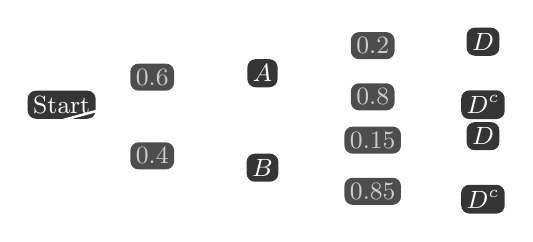
\begin{tikzpicture}[scale=1.0]
  \node[lab] at (0,1.2) {Start};
  \draw[base] (0,1.0)--(2.2,1.6);
  \draw[base] (0,1.0)--(2.2,0.4);
  \node[lab] at (2.55,1.6) {$A$};
  \node[lab] at (2.55,0.4) {$B$};
  \node[labm] at (1.15,1.55) {$0.6$};
  \node[labm] at (1.15,0.55) {$0.4$};

  \draw[base] (2.9,1.6)--(5.0,2.0);
  \draw[base] (2.9,1.6)--(5.0,1.2);
  \node[lab] at (5.35,2.0) {$D$};
  \node[lab] at (5.35,1.2) {$D^c$};
  \node[labm] at (3.95,1.95) {$0.2$};
  \node[labm] at (3.95,1.30) {$0.8$};

  \draw[base] (2.9,0.4)--(5.0,0.8);
  \draw[base] (2.9,0.4)--(5.0,0.0);
  \node[lab] at (5.35,0.8) {$D$};
  \node[lab] at (5.35,0.0) {$D^c$};
  \node[labm] at (3.95,0.75) {$0.15$};
  \node[labm] at (3.95,0.10) {$0.85$};
\end{tikzpicture}
\end{StepDiagram}

\Step{2} Substitute:
\[
P(D)=0.6(0.2)+0.4(0.15)=0.12+0.06=0.18.
\]
\EqDiagram{$P(\text{defective})=0.18=18\%$.}

\[
\boxed{0.18 \text{ (i.e., } 18\%\text{)}}
\]
\end{QAPair}

\end{document}
